%%%%%%%%%%%%%%%%%%%%
%                                             %
%                 Vernier Calipers            %
%                                             %
%%%%%%%%%%%%%%%%%%%%

\labChapter{}{Vernier Calipers}

The instrument illustrated in Fig.~\ref{VernierFig01} is a set of calipers.  The calipers have jaws $c$ and $d$ for measuring the diameter of a sphere or cylinder, $A$, or the thickness of any object placed between them. The inside diameter of a cavity is measured with jaws $e$ and $f$.  The depth of a hole is measured with the depth gauge, $g$.  The latter, and jaws $f$ and $d$ form part of a slide on which is engraved an auxiliary scale, the \textsl{Vernier scale} $v$. The scale on the fixed part (which carries jaws $c$ and $e$) is called the main scale. Only the metric scales are shown in the drawing, although the instrument have both U.S.\ and metric main and Vernier scales.

\begin{figure}
  \begin{center}
    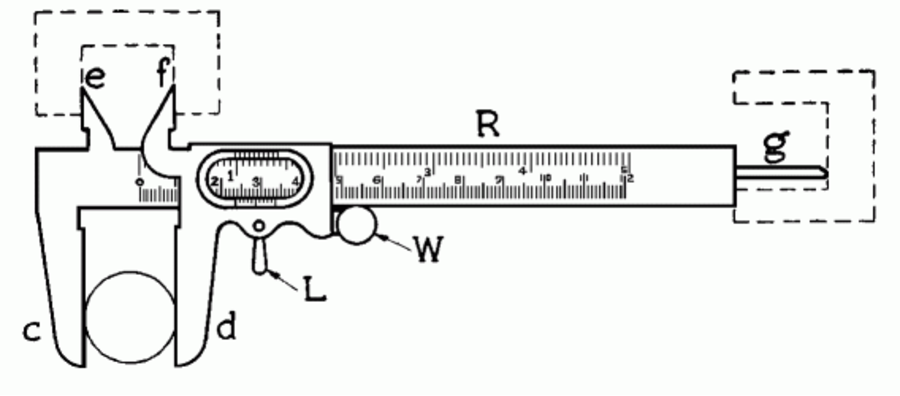
\includegraphics[width=5in]{IntroductionFigures/VernierCalipers01.pdf}
  \end{center}
  \caption{A diagram showing Vernier calipers and their main measurement scales.}
  \label{VernierFig01}  % the \label command comes AFTER the caption
\end{figure}

\section{Reading the Vernier scale}

Vernier scales, as used on the calipers and on many other types of high quality measuring instruments provide a means of reading accurately fractions of a scale division that otherwise have to be estimated.  In Fig.~\ref{VernierFig02}, we have illustrated a main scale with its Vernier scale.

\begin{figure}
  \begin{center}
    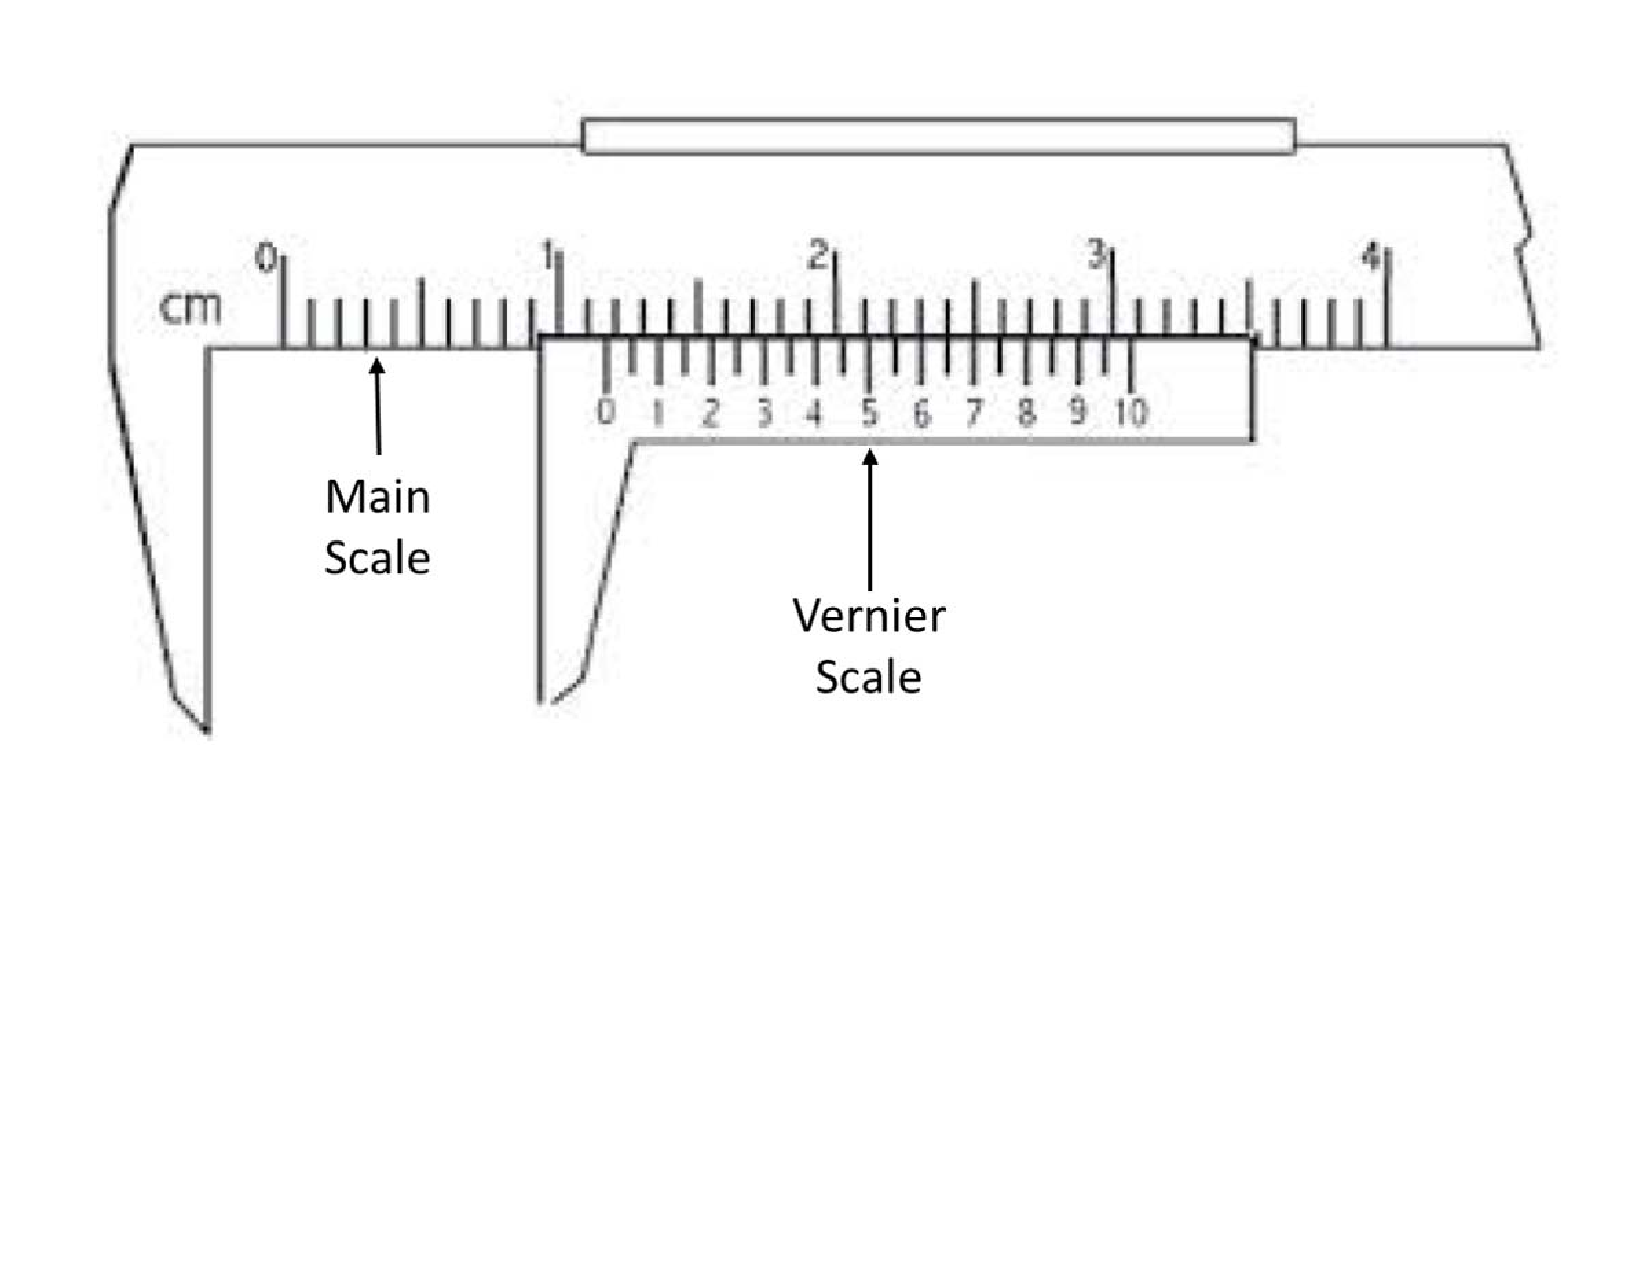
\includegraphics[width=5in]{IntroductionFigures/VernierCalipers02a.pdf}
  \end{center}
  \caption{How to read the value off the caliper slider.}
  \label{VernierFig02}  % the \label command comes AFTER the caption
\end{figure}

If each division on the main scale is $1\,\centi\meter$, then each division of the Vernier scale represents $1.0\,\milli\meter$.  Physically, it is a $9\,\milli\meter$ length divided into 10 equal parts. As an example, in the metric scale of Fig.~\ref{VernierFig02} the zero of the upper or Vernier scale is between the $1$ and $2\,\centi\meter$ marks on the main scale.  In this way, the Vernier scale is capable of interpolating to the nearest \milli\meter, the position of the Vernier zero mark on the main scale.  In this example, the measurement is  $1\,\centi\meter + \mbox{some number of \milli\meter}$.  In order to determine the number of \milli\meter, we read the number on the Vernier scale whose line coincides with a \centi\meter division line on the main scale.  (If the zero line of the Vernier is exactly on a division line of the main scale, then the measurement is exactly the main scale division.)  In this example, the division of the Vernier scale that lines up with a main scale division is the $0.7\,\milli\meter$ division.  The measurement would be $1.17\,\centi\meter$. You might have the situation where there is no exact alignment.  If that occurs, then you would estimate to the nearest $0.5\,\milli\meter$.  For example, if the $7\,\milli\meter$ division was slightly above and the $8\,\milli\meter$ division was slightly below corresponding marks on the main scale, then the measurement would be $1.175\,\centi\meter$.  Thus the Vernier scale is capable of estimating to the nearest $0.05\,\milli\meter$.  The rule for this type of Vernier therefore is to read the number of whole main scale divisions below the zero line of the Vernier, and in the next place of decimals insert the number of the line on the Vernier scale which coincides with a main scale line.

The smallest quantity, which may be read without estimating, is known as the least count; this is $1\,\milli\meter$ for the Vernier calipers illustrated.  For the Vernier calipers you will use in the laboratory, the least count is $0.1\,\milli\meter$.  In general, if the smallest division of the main scale of an instrument is $M$ units, and the length of the smallest Vernier division is $V$ units, then the least count, $L$, is $M V$. Also, since $n$ Vernier divisions are equal in length to $n-1$ main scale divisions,
\[
   nV = (n-1)M
\]
or
\[
   V = \frac{(n-1)M}{n}
\]
and thus
\[
   L = M - V = M - \frac{(n-1)M}{n} = \frac{M}{n}.
\]
